\documentclass{beamer}

\usepackage[T2A]{fontenc} % Выбор кодировки шрифтов
\usepackage[utf8]{inputenc} % Кодировка исходного текста (utf8)
\usepackage[english, russian]{babel} % Подключение языков (русский - основной)
\usepackage{tikz}
\usetikzlibrary{positioning}

\usetheme{Copenhagen} % Используем стандартную тему
\usecolortheme{whale}
\title{Навигация и картография робота по линиям и стрелочным символам}
\author{Перепечаев Виктор, Артур Адамов \\ Ментор: Николай Кузнецов}
\title[Навигация робота по линиям]{Навигация и картография робота по линиям и стрелочным символам}
\author[В. Перепечаев, А. Адамов]{Перепечаев Виктор, Артур Адамов \\ Ментор: Николай Кузнецов}
\date{\today}

\begin{document}

\begin{frame}
    \titlepage
\end{frame}

\begin{frame}{Содержание}
    \tableofcontents
\end{frame}

\section{МТС True Tech Champ}
\begin{frame}{Первый Этап}
    \begin{columns}[onlytextwidth, T] % [T] выравнивает колонки по верхнему краю
        \begin{column}{0.5\textwidth} % Левая колонка для текста (50% ширины)
            \textbf{Дано:}
            \begin{itemize}
                \item Маленькая виртуальная комната с препятствиями
                \item Интерфейс для управления роботом в этой комнате
            \end{itemize}
            \textbf{Задача:}
            Довести робота от старта до финиша
        \end{column}
        \begin{column}{0.45\textwidth} % Правая колонка для картинки (45% ширины)
            \centering
            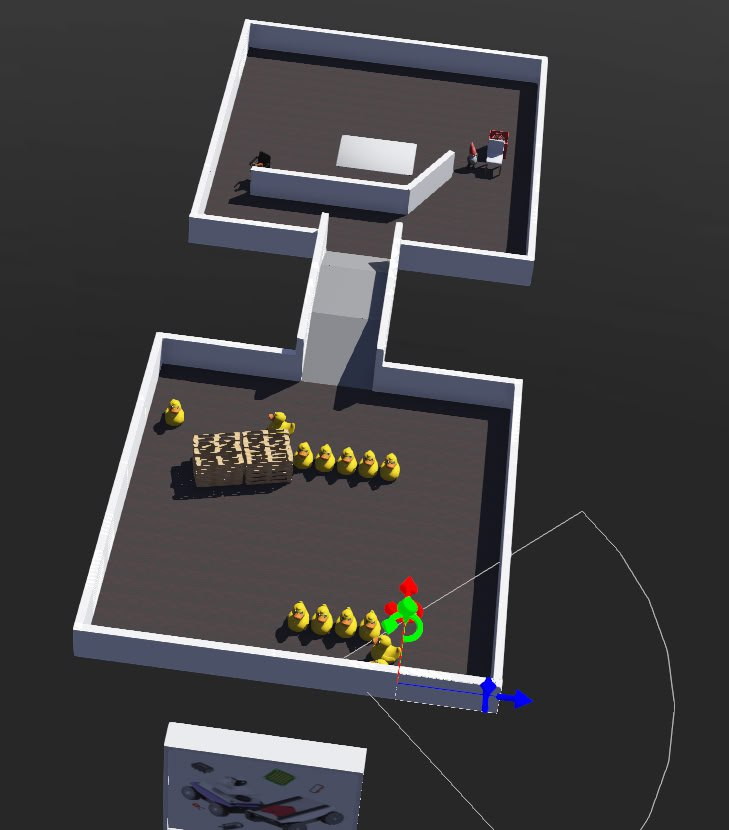
\includegraphics[width=\linewidth]{ducks_room.jpg} % Картинка на всю ширину колонки
            %\caption{Виртуальная тестовая комната} % Опциональная подпись
        \end{column}
    \end{columns}
\end{frame}

\begin{frame}{Первый Этап}
  \textbf{Решение:}
  \begin{enumerate}
    \item Написали простой контроллер
    \item Собственными руками провели робота до финиша
    \item Сохранили все отправленные роботу команды
  \end{enumerate}
  \vspace{5mm}
  \textbf{Итог:}
  Прошли дальше
\end{frame}

\begin{frame}{Второй Этап}
    \begin{columns}[onlytextwidth, T] % [T] выравнивает колонки по верхнему краю
        \begin{column}{0.5\textwidth} % Левая колонка для текста (50% ширины)
            \textbf{Дано:}
            \begin{itemize}
                \item Большой виртуальный лабиринт с препятствиями
                \item Интерфейс для управления роботом в этом лабиринте
            \end{itemize}
            \textbf{Задача:}
            Робот должен автономно доехать из угла в центр при неизвестной изначальной конфигурации лабиринта
        \end{column}
        \begin{column}{0.45\textwidth} % Правая колонка для картинки (45% ширины)
            \centering
            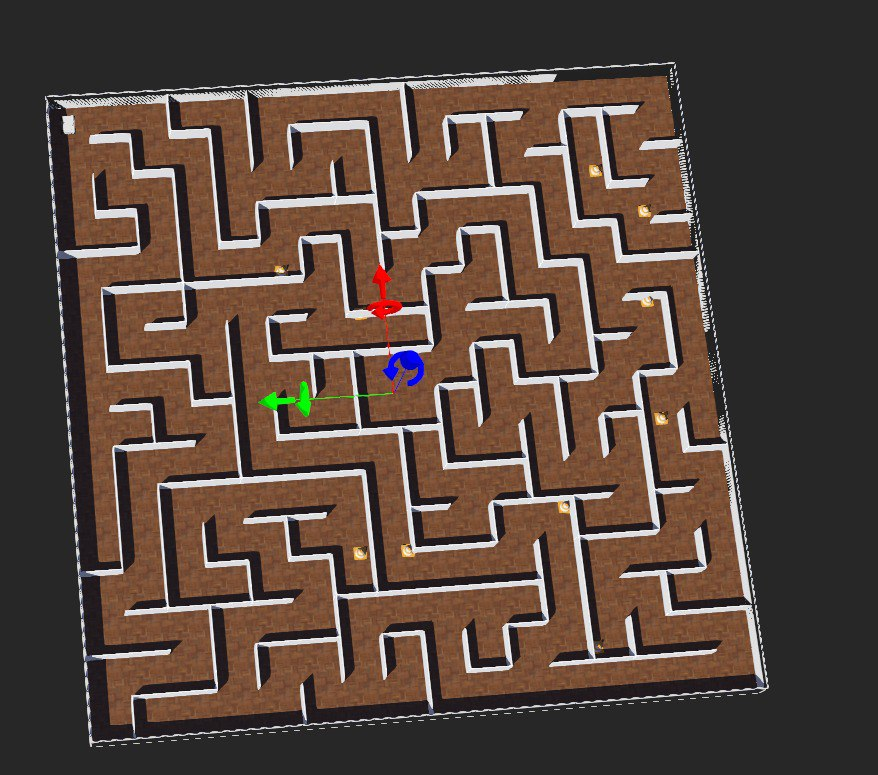
\includegraphics[width=\linewidth]{Labyrinth.jpg} % Картинка на всю ширину колонки
            %\caption{Виртуальная тестовая комната} % Опциональная подпись
        \end{column}
    \end{columns}
\end{frame}
\begin{frame}{Второй этап.Решение: стек технологий}
    \centering
    % Простая схема стека (можно заменить на реальную картинку)
    \begin{tikzpicture}[node distance=0.7cm]
        \node[draw, fill=blue!20, minimum width=8cm, minimum height=1cm, rounded corners] (webots) {\textbf{Уровень симуляции: Webots}};
        \node[draw, fill=green!20, minimum width=8cm, minimum height=1cm, rounded corners, below=of webots] (ros) {\textbf{Уровень связи и управления: ROS 2 (Humble)}};
        \node[draw, fill=orange!20, minimum width=8cm, minimum height=1cm, rounded corners, below=of ros] (slam) {\textbf{Уровень навигации: SLAM Toolbox}};
        \node[draw, fill=red!20, minimum width=8cm, minimum height=1cm, rounded corners, below=of slam] (viz) {\textbf{Уровень визуализации: RViz}};
        \draw[<->, thick] (webots.south) -- (ros.north);
        \draw[<->, thick] (ros.south) -- (slam.north);
        \draw[<->, thick] (slam.south) -- (viz.north);
    \end{tikzpicture}
\end{frame}
\begin{frame}{Второй этап.Решение: Пример}
    %\begin{column}{0.8\textwidth} % Правая колонка для картинки (45% ширины)
        \centering
        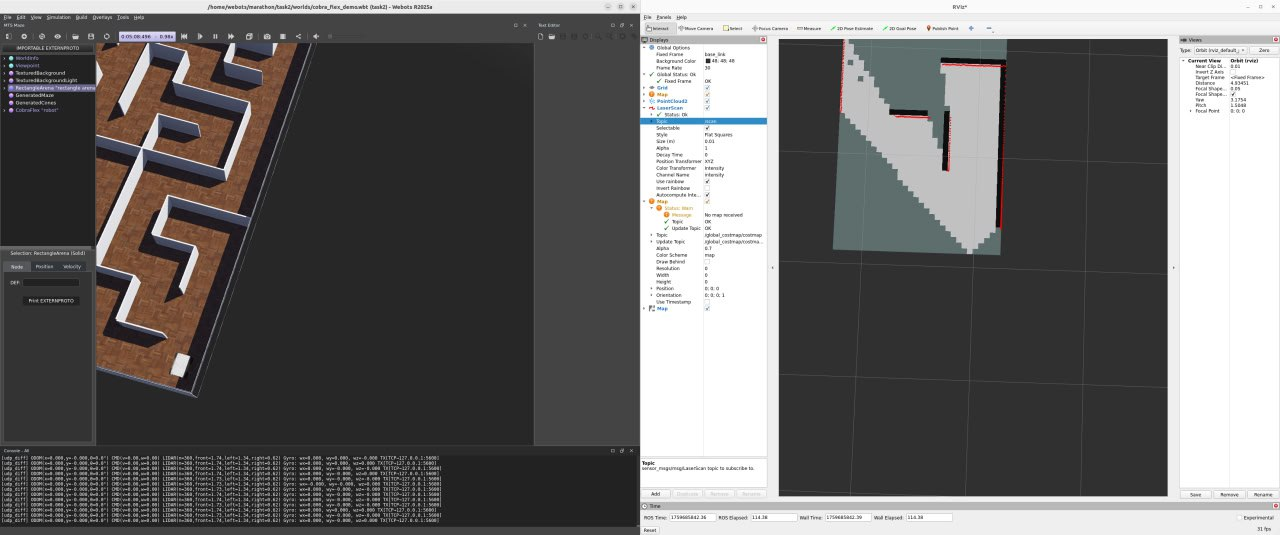
\includegraphics[width=\linewidth]{workflow.jpg} % Картинка на всю ширину колонки
        %\caption{Виртуальная тестовая комната} % Опциональная подпись
    % \end{column}
\end{frame}
\begin{frame}{Второй этап.Решение}
  \textbf{Итог:} Прошли
\end{frame}

\begin{frame}{Третий Этап}
    \begin{columns}[onlytextwidth, T] % [T] выравнивает колонки по верхнему краю
        \begin{column}{0.5\textwidth} % Левая колонка для текста (50% ширины)
            \textbf{Дано:}
            \begin{itemize}
                \item Маленький физический лабиринт
                \item Интерфейс для управления физическим роботом по ssh
            \end{itemize}
            \textbf{Задача:}
            Робот должен автономно проехать от старта до финиша
        \end{column}  
        \begin{column}{0.45\textwidth} % Правая колонка для картинки (45% ширины)
            \centering
            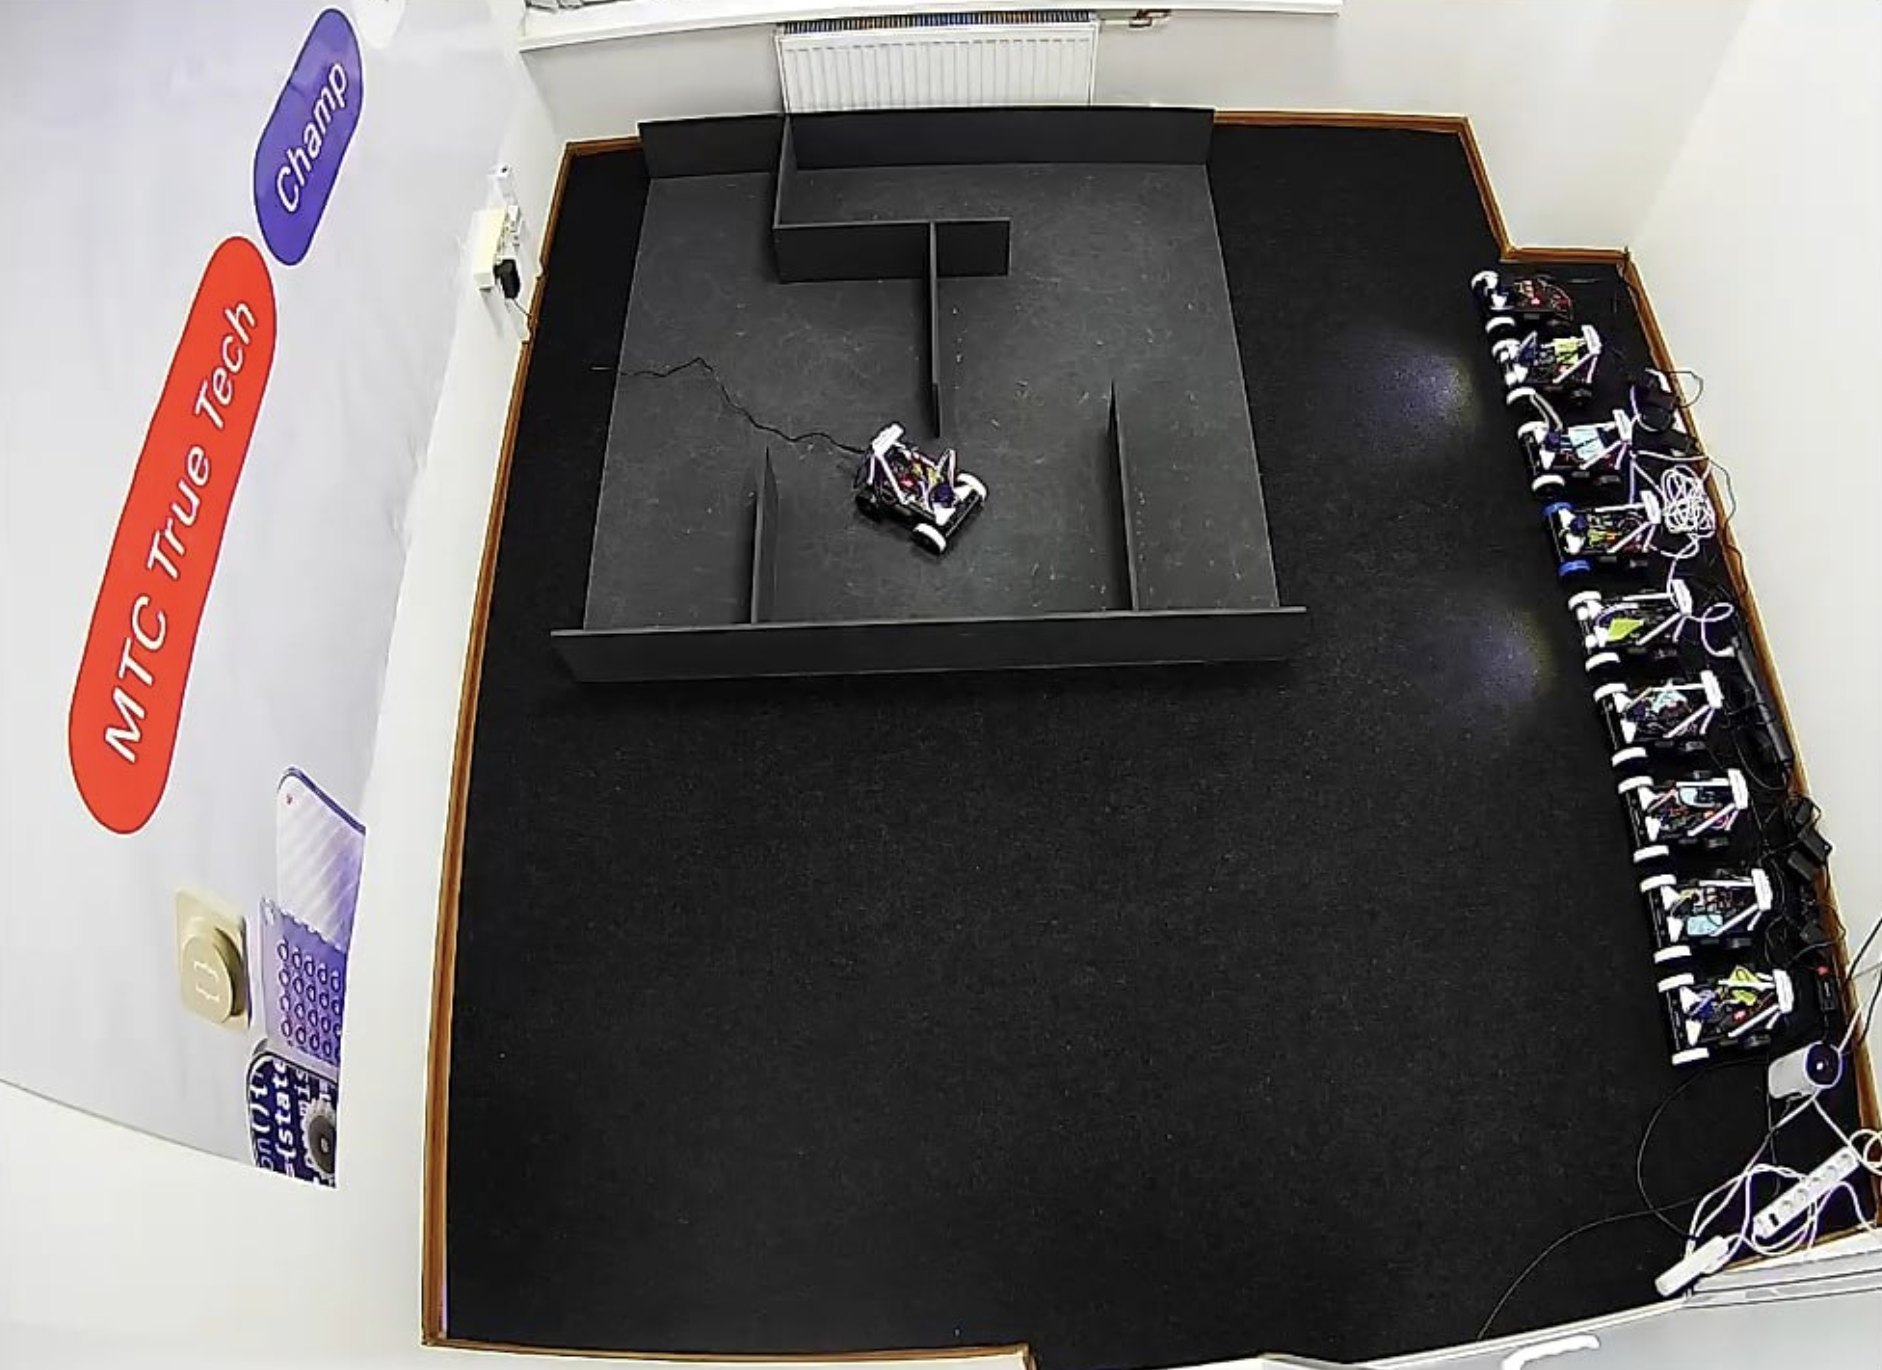
\includegraphics[width=\linewidth]{robots_station.png} % Картинка на всю ширину колонки
            %\caption{Виртуальная тестовая комната} % Опциональная подпись
        \end{column}
    \end{columns}
\end{frame}

\begin{frame}{Третий этап}
  \textbf{Итог:} Не прошли\\
  \vspace{5mm}
  \textbf{Причины:}
  \begin{itemize}
    \item Уменьшение команды
    \item Большое кол-во дедлайнов в МФТИ
    \item Трудности по доступу к/настройке робота
  \end{itemize}
\end{frame}

\section{Картография}
\begin{frame}{Постановка}
    \begin{columns}[onlytextwidth, T] % [T] выравнивает колонки по верхнему краю
        \begin{column}{0.5\textwidth} % Левая колонка для текста (50% ширины)
            \textbf{Дано:}
            \begin{itemize}
                \item Поле с ярко-красной изолентой
                \item Гуманоидный робот
                \item Запись с камер робота
            \end{itemize}
            \textbf{Задача:}
            Восстановить траекторию движения робота в физическом мире
        \end{column}  
        \begin{column}{0.45\textwidth} % Правая колонка для картинки (45% ширины)
            \centering
            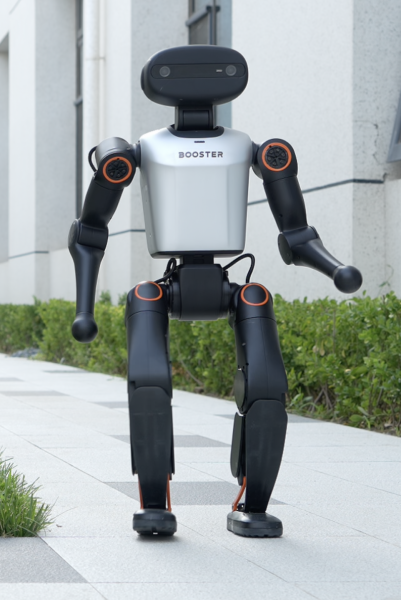
\includegraphics[width=0.8\linewidth]{booster_k1.png} % Картинка на всю ширину колонки
            %\caption{Виртуальная тестовая комната} % Опциональная подпись
        \end{column}
    \end{columns}
\end{frame}

\begin{frame}{Решение.IMU}
  Опр: IMU - Internal Measuremnt Unit
  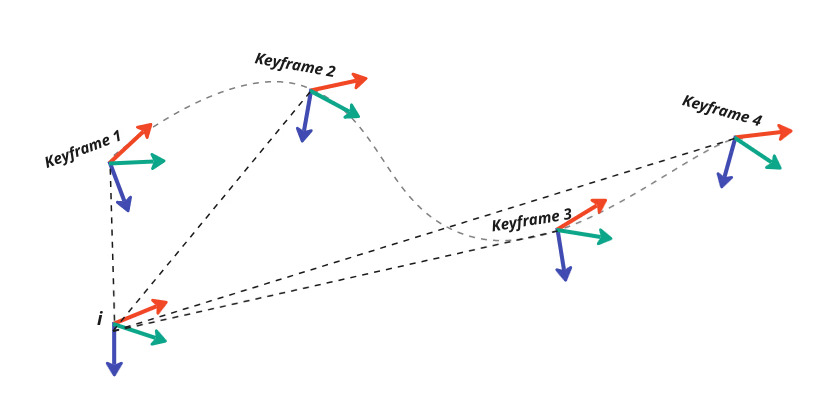
\includegraphics[width=\linewidth]{imu_preintegration.jpg}
\end{frame}
\begin{frame}{Решение.CV}
  \centering
    % Основной контейнер для картинок с подписями
    \begin{tikzpicture}[node distance=0.5cm]
        % ЛЕВАЯ КАРТИНКА с подписью
        \node (img1) [inner sep=0pt] {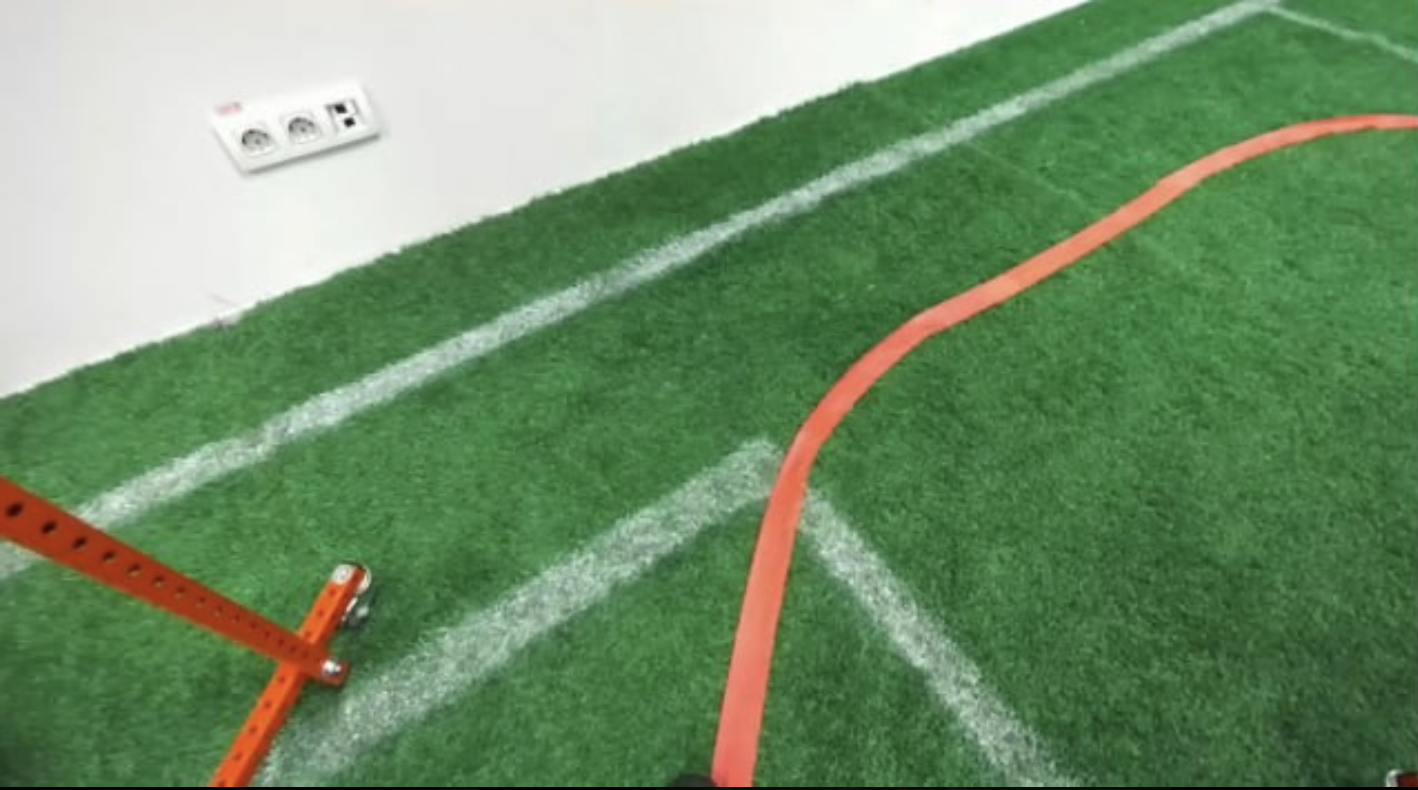
\includegraphics[width=0.4\linewidth]{cv_input.png}};

        % СТРЕЛКА
        \node (arrow) [right= of img1] {\huge $\Rightarrow$}; % Можно заменить на ->, →, \rightarrow

        % ПРАВАЯ КАРТИНКА с подписью
        \node (img2) [right= of arrow, inner sep=0pt] {
\includegraphics[width=0.4\linewidth]{cv_output.png}};
    \end{tikzpicture}
\end{frame}
\begin{frame}{Решение.Текущие результаты}
  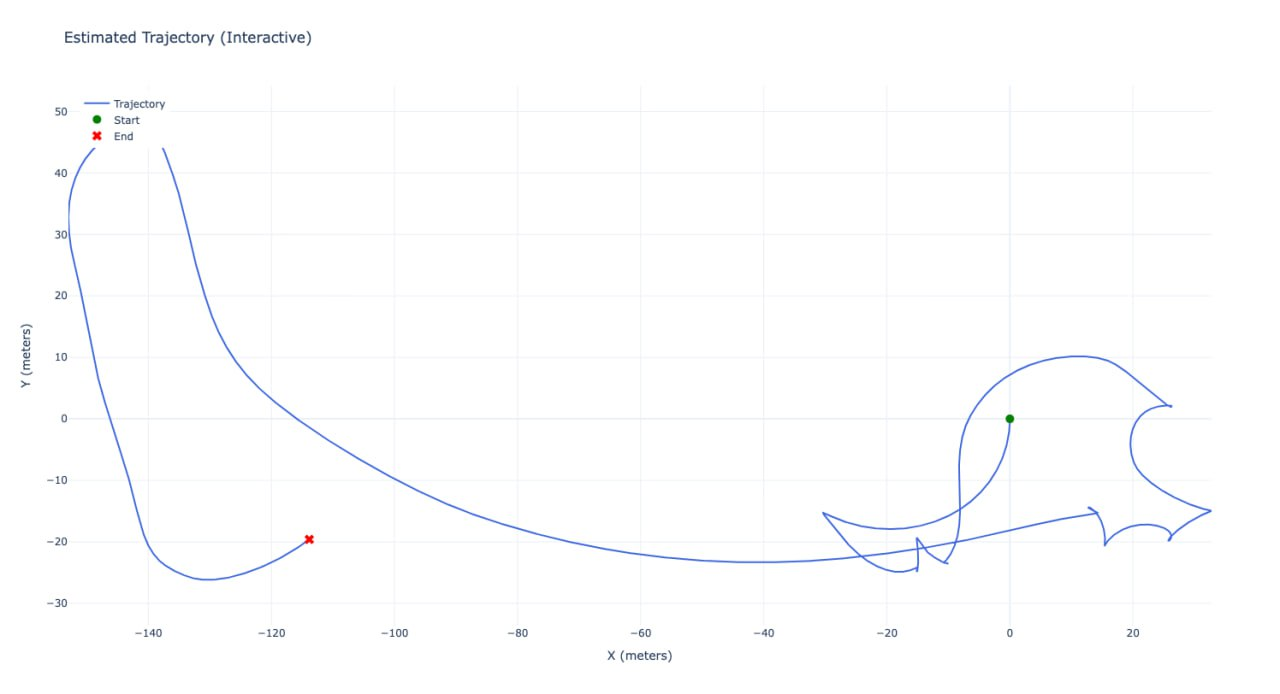
\includegraphics[width=\linewidth]{result_without_imu.jpg}
\end{frame}
\begin{frame}{Решение.Текущие результаты}
  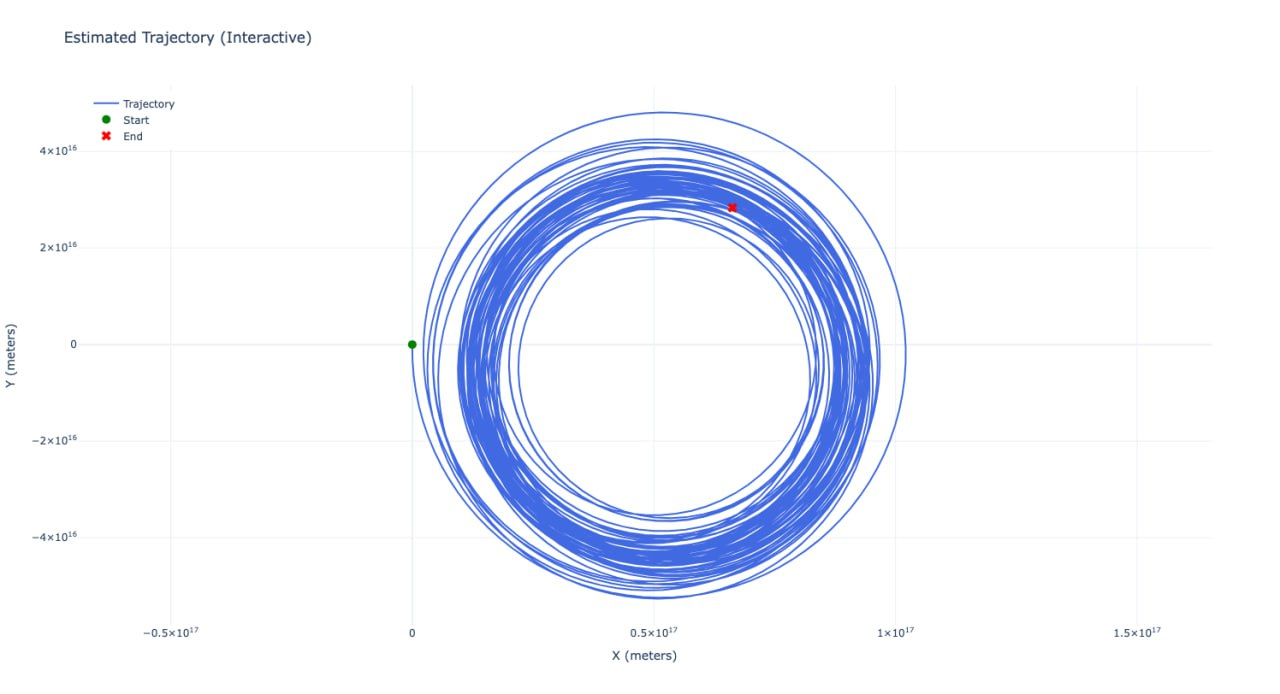
\includegraphics[width=\linewidth]{result_with_imu.jpg}
\end{frame}

\section{Выводы}
\begin{frame}{Выводы: что мы получили от проекта}
    \begin{block}{Приобретённые компетенции и инструменты}
        \begin{itemize}
            \item Практический опыт работы с промышленным стеком: \textbf{ROS 2 Humble, RViz, SLAM Toolbox}.
            \item Углубили навыки в области \textbf{компьютерного зрения}.
            \item Освоили принципы интеграции разнородных данных (видео, IMU) для построения согласованной картины мира.
        \end{itemize}
    \end{block}
\end{frame}

\section{Планы}
\begin{frame}{Планы по развитию проекта}
    \centering
    \begin{columns}[T, onlytextwidth]
        \begin{column}{0.32\textwidth}
            \textbf{Алгоритм:}
            \begin{itemize}\footnotesize
                \item Повысить точность восстановления траектории.
                \item Добавить фактор граф-сетов (Pose Graph) для коррекции дрейфа.
                \item Восстанавливать траекторию в реальном времени.
            \end{itemize}
        \end{column}
        \begin{column}{0.32\textwidth}
            \textbf{Внедрение:}
            \begin{itemize}\footnotesize
                \item Протестировать в условиях различного освещения и помех.
            \end{itemize}
        \end{column}
        \begin{column}{0.32\textwidth}
            \textbf{Функционал:}
            \begin{itemize}\footnotesize
                \item Научить робота читать знаки на поле.
                \item Реализовать простые сценарии взаимодействия (например, "следуй к объекту X").
            \end{itemize}
        \end{column}
    \end{columns}
\end{frame}

\begin{frame}
    \centering
    \Huge Спасибо за внимание!
\end{frame}

\end{document}